\chapter{\scshape Elements of vertical mixing schemes}
\label{chapter:cvmix_elements}

\minitoc
\vspace{.5cm}

This chapter presents certain of the elements required for computing
various CVMix parameterization schemes.  Details specific to
particular schemes are provided in later chapters.

\section{Discrete vertical grid}
\label{section:vertical-grid-numerics}

As part of the numerical discretizations used by CVMix modules, we
have need to describe how discrete fields are placed on a vertical
grid, and how finite difference operations are performed.  A vertical
column generally has time dependent positions of the discrete fields,
distances between the positions, and thicknesses of the cells over
which the discrete fields are defined.  Generality is necessary for
models where grid cell thicknesses are functions of time, and CVMix
allows for such freedom.

Figure \ref{fig:cvmix_discrete_vertical} provides a schematic of the
conventions for a tracer column used by CVMix modules. The conventions
are motivated by those used in MOM and POP, yet some details may
differ slightly.  A summary of the choices made in developing this
figure are as follows.
\begin{itemize}

\item {\sc vertical coordinate}: The vertical coordinate $z$ increases
  upward and extends from the ocean bottom at $z=-H(x,y)$ to the sea
  surface at $z = \eta(x,y,t)$.

\item {\sc tracer cell arrays}: Tracer cell arrays are labelled with
  the discrete index {\tt kt}, and have dimensions {\tt nlevs}.  The
  index {\tt kt} increases downward starting from {\tt kt} =1 for the
  top model grid cell.  The number of levels, {\tt nlevs}, is a
  function of the column, with only wet points included in a CVMix
  column.  Examples of tracer cell arrays include temperature,
  salinity, pressure, density, thermal expansion coefficient, and
  haline contraction coefficient.

\item {\sc w-cell or interface arrays}: W-cell or interface arrays are
  labelled with the discrete index {\tt kw}, and have dimensions {\tt
    nlevs+1}.  The index {\tt kw} increases downward starting from
  {\tt kw} =1 at the top ocean interface.  The notation ``w-cell''
  originates from the continuity equation, in which the vertical
  velocity component, $w$, transfers mass across the vertical
  interfaces of tracer cells.  Examples of w-cell or interface arrays
  are diffusivity, viscosity, vertical tracer derivatives, buoyancy
  frequency, and Richardson number.  For most w-cell arrays, both the
  top interface at {\tt kw=1} and bottom interface at {\tt kw=nlevs+1}
  have zero values.

  One argument for using {\tt nlevs+1} interfaces is that we avoid
  ambiguity of where the data resides. Interface arrays of size {\tt
    nlevs} could start at either the top or bottom of the first level
  and, despite documentation, the ambiguity will increase the
  potential for code errors.  It does not matter so much whether
  interface arrays are dimensioned {\tt 0:nlevs} or {\tt 1:nlevs+1};
  there is only one way the data could be laid out relative to the
  tracer arrays which have dimensions {\tt 1:nlevs}. Yet the reason to
  prefer {\tt 1:nlevs+1} is that this dimensioning simplifies
  declarations and argument passing, given the standard assumptions
  made by Fortran in laying out memory for arrays.

 
\item {\sc tracer cell thickness}: The rectangular boxes in Figure
  \ref{fig:cvmix_discrete_vertical} represent tracer cells whose
  thickness is measured by the array element {\tt dzt(kt)} with units
  of meter. This array has dimensions {\tt dzt(nlevs)}.  These
  thicknesses are generally time dependent.  The array {\tt dzt} is an
  input to CVMix, passed from the ocean model each time step.

\item {\sc w-cell thickness or tracer point separation}: The array
  {\tt dzw} has dimensions {\tt dzw(nlevs+1)}.  The array element {\tt
    dzw(kw=1)} measures distance (in meters) from the top of the top
  tracer cell to the tracer point {\tt T(kt=1)}, and array element
  {\tt dzw(kw=nlevs+1)} measures the distance from the bottom tracer
  point {\tt T(kt=nlevs)} to the bottom of the bottom tracer cell.
  Intermediate elements of {\tt dzw} measure the distance between
  tracer points, or equivalently the thickness of a w-cell.  These
  distances are generally time dependent.  The array {\tt dzw} is an
  input to CVMix, passed from the ocean model each time step.

\item {\sc distance from ocean surface to tracer cell point}: The
  distance (in meters) from the tracer cell point to the ocean surface
  is given by the array element {\tt zt(kt)}.  This array has
  dimensions {\tt zt(nlevs)}.  If needed, the array {\tt zt} is
  constructed inside CVMix code based on the values of {\tt dzt} and
  {\tt dzw}. 

\item {\sc distance from ocean surface to interface}: The distance
  from the tracer cell interface, or the w-point, to the ocean surface
  is given by the array element {\tt zw(kw)}.  This array has
  dimensions {\tt zw(nlevs+1)}.  If needed, the array {\tt zw} is
  constructed inside CVMix code based on the values of {\tt dzt} and
  {\tt dzw}.

\end{itemize}



%%%%%%%%%%%%%%%%%%%% %%%%%%%%%%%%%%%%%%%%%%%%%
\begin{figure}[h!t]
\begin{center}
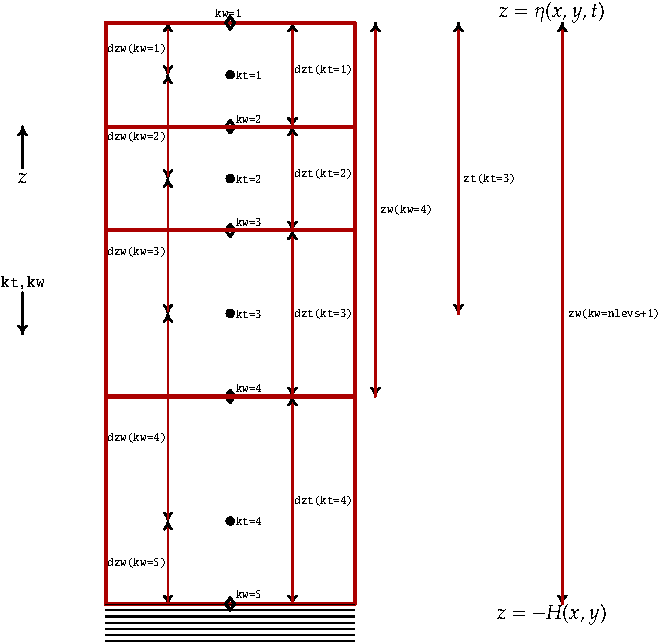
\includegraphics[angle=0,width=10cm]{./mfpic_figs/cvmix_discrete_vertical.pdf}
\caption[Discrete vertical column for CVMix modules]{\sf Schematic of
  a discrete vertical column used in CVMix modules, with the surface
  at $z=\eta(x,y,t)$ and bottom at $z=-H(x,y)$.  The vertical
  coordinate $z$ increases upward, whereas the discrete vertical
  indices {\tt kt} and {\tt kw} increase downward.  CVMix code assumes
  distances and thicknesses are in units of meters. The rectangular
  boxes represent tracer cells in the ocean model.  The array element
  {\tt dzt(kt)} measures the thickness of a tracer cell. This array
  has dimensions {\tt dzt(nlevs)}, where {\tt nlevs} is the number of
  wet cells in a particular column.  For this particular example, {\tt
    nlevs} = 4.  The array {\tt dzw} has dimensions {\tt
    dzw(nlevs+1)}.  The array element {\tt dzw(kw=1)} measures the
  distance from the top of the top tracer cell to the tracer point
  {\tt T(kt=1)}, and array element {\tt zw(kw=nlevs+1)} measures the
  distance from the bottom tracer point {\tt T(kt=nlevs)} to the bottom
  of the bottom tracer cell.  Intermediate elements of {\tt dzw}
  measure the distance between tracer points, or equivalently the
  thickness of w-cells.  The distance from the ocean surface to a
  tracer point is measured by the array element {\tt zt(kt)}, and the
  distance to the interface is measured by {\tt zw(kw)}.  The total
  thickness of a column is {\tt zw(nlevs+1)}, and it is generally time
  dependent, as are all of the grid distances {\tt dzt} and {\tt dzw}.
  Arrays that are defined at the interface, such as buoyancy
  frequency, Richarson number, diffusivity, viscosity, have vertical
  indices {\tt kw}.  Arrays defined at the tracer cell point, such as
  temperature, salinity, and density, have vertical indices {\tt kt}.}
\label{fig:cvmix_discrete_vertical}
\end{center}
\end{figure}
%%%%%%%%%%%%%%%%%%%%%%%%%%%%%%%%%%%%%%%%%%%%%%%%%%%%%%%%%%%%%%%%%%%%%%%%


\section{Gravitational stability}
\label{section:buoyancy-frequency-elements}

Buoyancy stratification plays a key role in ocean physical proceses.
We have need to quantify stratification, and the associated
gravitational stability of a water column.  For this purpose, we
introduce the notion of an adiabatic and isohaline parcel
displacement, from which we develop an algorithm for computing the
buoyancy frequency used to measure vertical stratification.  The
notions detailed here should be respected by the calling ocean model
in order for the CVMix modules to produce physically relevant results.
\begin{quote}
  {\sf The squared buoyancy frequency, $N^2$, is an input to CVMix
    modules.}
\end{quote}


\subsection{Infinitesimal displacements}

Consider an infinitesimal displacement $\mathrm{d}{\bf x}$ of a fluid
parcel.  The {\it in situ} density at the new point is related to the
reference density by
\begin{equation}
 \rho({\bf x} + \mathrm{d} \, {\bf x})= \rho({\bf x}) + \mathrm{d}\rho({\bf x}).
\end{equation}
Using a Taylor series expansion, the density increment can be
approximated by
\begin{equation}
\begin{split}
\mathrm{d}\rho &=  \mathrm{d}{\bf x} \cdot \nabla \rho
 \\
 &= \rho \, \mathrm{d}{\bf x} \cdot \rho^{-1} \, \nabla \rho
\\
&= 
\rho \, \mathrm{d}{\bf x} \cdot 
 \left( -\alpha \, \nabla \Theta + \beta \, \nabla  S  + \frac{\nabla p}{\rho \, c_{\mbox{\tiny sound}}^{2}  } \right),
\end{split}
\label{eq:full-density-increment-displacement}
\end{equation}
where all terms on the right hand side are evaluated at the reference
point ${\bf x}$.  To reach this expression, we introduced the thermal
expansion coefficient
\begin{equation}
 \alpha = -\frac{1}{\rho}\left( \frac{\partial \rho}{\partial \Theta} \right),
\label{eq:alpha-elements}
\end{equation}
the haline contraction coefficient 
\begin{equation}
 \beta = \frac{1}{\rho}\left( \frac{\partial \rho}{\partial S} \right),
\label{eq:beta-elements}
\end{equation}
and the squared sound speed
\begin{equation}
 c^{2}_{\mbox{\tiny sound}} = \left( \frac{\partial p}{\partial \rho}\right).
\label{eq:sound-speed-elements}
\end{equation}
The ambient density at the new point, $\rho({\bf x} + \mathrm{d} {\bf
  x})$, thus differs from density at the reference point, $\rho({\bf
  x})$, by an amount $\mathrm{d}\rho({\bf x})$ according to
\begin{equation}
 \rho({\bf x} + \mathrm{d} \, {\bf x}) - \rho({\bf x}) = 
 \rho({\bf x}) \, \mathrm{d}{\bf x} \cdot 
 \left( -\alpha \, \nabla \Theta + \beta \, \nabla  S  + \frac{ \nabla p }{\rho \, c_{\mbox{\tiny sound}}^{2}  }\right).
\end{equation}


\subsection{Neutral directions}
\label{subsection:neutral-directions}

Displacements that allow for temperature and salinity to change
require energy for mixing to occur.  Such energy can arise from
various sources, such as astronomical tides \citep{MunkWunsch98}. We
are not concerned here with such energy sources.  Instead, we wish to
know if through buoyancy forces alone a particular parcel displacement
is favored, resisted, or neutral.  For this purpose, we introduce the
notion of a displacment restricted to adiabatic and isohaline
conditions (i.e., no heat or salt exchanged during the parcel
displacement).  Such fictitious displacements occur in the absence of
energy needed for mixing, and so they are useful to explore where
parcel motions may signal a fluid instability associated with buoyancy
forces.

The density change associated with an adiabatic and isohaline
displacement is determined just by pressure changes arising from the
displacement, so that
\begin{equation}
\rho({\bf x} + \mathrm{d} {\bf x})_{\mbox{\tiny  adiabatic/isohaline}} - \rho({\bf x})  =
  \rho \, \mathrm{d}{\bf x} \cdot  \left( \frac{ \nabla p }{\rho \, c_{\mbox{\tiny sound}}^{2}  } \right).
\label{eq:infinitesimal-rho-adiabatic}
\end{equation}
This density change occurs merely through the pressure dependence of
{\it in situ} density.  Operationally, to compute $\rho({\bf x} +
\mathrm{d} {\bf x})_{\mbox{\tiny adiabatic/isohaline}}$, we may choose
to evaluate the right hand side of equation
(\ref{eq:infinitesimal-rho-adiabatic}), or we may evaluate the
equation of state at the temperature and salinity of the reference
point, ${\bf x}$, but with pressure at the displaced point, ${\bf x} +
\mathrm{d} {\bf x}$
\begin{equation}
  \rho({\bf x} + \mathrm{d} {\bf x})_{\mbox{\tiny adiabatic/isohaline}} 
 = \rho[ \Theta({\bf x}), S({\bf x}), p({\bf x}  + \mathrm{d} {\bf x})]. 
\end{equation}
The difference in density between a parcel undergoing an adiabatic and
isohaline displacement, $\rho({\bf x} + \mathrm{d} {\bf x})_{\mbox{\tiny
    adiabatic/isohaline}}$, and the density of the ambient environment,
$\rho({\bf x} + \mathrm{d} {\bf x})$, is thus given by
\begin{equation}
\begin{split}
\rho({\bf x} + \mathrm{d} {\bf x})  - \rho({\bf x} + \mathrm{d} {\bf x})_{\mbox{\tiny  adiabatic/isohaline}} 
&=
\rho[ \Theta({\bf x} + \mathrm{d} {\bf x}), S({\bf x} + \mathrm{d} {\bf x}), p({\bf x} + \mathrm{d} {\bf x})]
-
\rho[ \Theta({\bf x} ), S({\bf x}), p({\bf x} + \mathrm{d} {\bf x})]
\\
&= 
  \rho \, \mathrm{d}{\bf x} \cdot 
  \left( -\alpha \, \nabla \Theta + \beta \, \nabla  S \right).
\end{split}
\label{eq:neutral-directions-motivated}
\end{equation}
If a parcel makes an adiabatic and isohaline excursion and finds
itself in a region where the ambient density is unchanged, then there
are no buoyancy forces to resist that displacement.  Directions
defined by such displacements are termed {\it neutral directions}
\citep{McDougall1987a}.  By definition, neutral directions are
orthogonal to the local dia-neutral unit vector
\begin{equation}
 \hat{\gamma} = \left( \frac{-\alpha \, \nabla \Theta + \beta \, \nabla S}
                          {|-\alpha \, \nabla \Theta + \beta \, \nabla S|}
 \right),
\end{equation}
 so that 
\begin{equation}
\rho({\bf x} + \mathrm{d} {\bf x})  - \rho({\bf x} + \mathrm{d} {\bf x})_{\mbox{\tiny  adiabatic/isohaline}} 
 = 
 \left( \rho \, \mathrm{d}{\bf x} \cdot \hat{\gamma} \right) \, 
 |-\alpha \, \nabla \Theta + \beta \, \nabla  S |. 
\end{equation}


\subsection{Squared buoyancy frequency}
\label{subsection:buoyancy-frequency-and-stability}

When measuring the gravitational stability of a fluid column, we are
concerned with vertical displacements and the resistence from buoyancy
stratification to such displacements.  To anticipate the needs of the
discrete calculation, we assume knowledge of the density, tracer
concentration, and pressure at depths $z$ and $z+\mathrm{d}z$ (see
Figure \ref{fig:cvmix_stability}).


\subsubsection{Stability to upward displacements from a deeper reference point}

Consider first an upward displacement starting from the reference
depth $z$ and going to $z+\mathrm{d}z$.  Following the notation of
Figure \ref{fig:cvmix_stability}, we have
\begin{equation}
\rho(z+\mathrm{d} z)  - \rho(z+\mathrm{d} z)_{\mbox{\tiny adiabatic/isohaline}}  
= 
 \rho[ \Theta(z + \mathrm{d} z), S(z + \mathrm{d} z), p(z + \mathrm{d} z)]
-
\rho[ \Theta(z), S(z), p(z + \mathrm{d}z)].
\end{equation}
As for the case of a general displacement considered in Section
\ref{subsection:neutral-directions}, we perform a Taylor series
expansion about the reference depth at $z$ to render the leading order
identity
\begin{equation}
\begin{split}
\rho(z+\mathrm{d} z)  - \rho(z+\mathrm{d} z)_{\mbox{\tiny adiabatic/isohaline}}  
&\approx 
  \rho(z) \, \mathrm{d}z \, \left[ 
   -\alpha(z) \, \left( \frac{\partial \Theta}{\partial z} \right )
 + \beta(z) \, \left( \frac{\partial S}{\partial z} \right) \right]
 \\
&= 
 -\left( \frac{\rho \, \mathrm{d}z}{g} \right) \, N^{2}.
\end{split}
\label{eq:inifinitesimal-delta-rho-elements-upwards1}
\end{equation}
The final equality in equation
(\ref{eq:inifinitesimal-delta-rho-elements-upwards1}) introduced the
squared buoyancy frequency
 \begin{equation}
 N^{2}_{\mbox{\scriptsize linear}} = g \, \left( \alpha \, \frac{\partial \Theta}{\partial z} 
                         - \beta  \, \frac{\partial S}{\partial z} \right),
\label{eq:buoyancy-frequency-elements}
\end{equation}
where the vertical derivatives and expansion coefficients are
evaluated at the deep reference point $z$.  Calculating gravitational
stability according to the linear approximate expresson
(\ref{eq:buoyancy-frequency-elements}) is accurate so long as all
higher order terms in the Taylor series approximation can be
neglected.  It is for this reason we denote this a linear
approximation to the buoyancy frequency.  The higher order terms are
potentially important in regions where the equation of state becomes
quite nonlinear, such as the high latitudes of the Southern Ocean.  So
we do not generally recommend this approximation for global modeling.
Instead, we recommend use of the full squared buoyancy frequency
\begin{equation}
\begin{split}
 N^{2}_{\mbox{\scriptsize full}}(z \rightarrow z+\mathrm{d}z) &\equiv 
 -\left( \frac{g \, [ \rho(z+\mathrm{d} z)  - \rho(z+\mathrm{d} z)_{\mbox{\tiny adiabatic/isohaline}} ] } {\rho(z) \, \mathrm{d}z} \right)
\end{split}
\label{eq:inifinitesimal-delta-rho-elements-upwards2}
\end{equation}

Again, the calculation
(\ref{eq:inifinitesimal-delta-rho-elements-upwards2}) will determine
gravitational stability of an upward parcel displacement from depth
$z$ to $z+\mathrm{d}z$.  To further expose the physics of this
calculation, consider two vertical stratifications.
\begin{itemize}
\item {\sc gravitationally stable stratification:
    $N^{2}_{\mbox{\scriptsize full}}(z \rightarrow z+\mathrm{d}z) >
    0$}: In this case, a vertically upward displacement occurring
  without heat or salt exchange will produce a parcel density that is
  more than the ambient density: $\rho(z+\mathrm{d} z) -
  \rho(z+\mathrm{d} z)_{\mbox{\tiny adiabatic/isohaline}} <0$. This
  particular adiabatic and isohaline displacement is resisted by
  buoyancy forces.  The vertical density profile is thus
  gravitationally stable.

\item {\sc gravitationally unstable stratification:
    $N^{2}_{\mbox{\scriptsize full}}(z \rightarrow z+\mathrm{d}z) <
    0$}: Now the upward adiabatic and isohaline displacement leads to
  a lesser density than the ambient environment: $\rho(z+\mathrm{d} z)
  - \rho(z+\mathrm{d} z)_{\mbox{\tiny adiabatic/isohaline}} >0$.  This
  particular adiabatic and isohaline displacement is encouraged by
  buoyancy forces to rise even further. The vertical density profile
  is thus gravitationally unstable.

\end{itemize}

\begin{figure}
\begin{center}
\resizebox{5cm}{!}{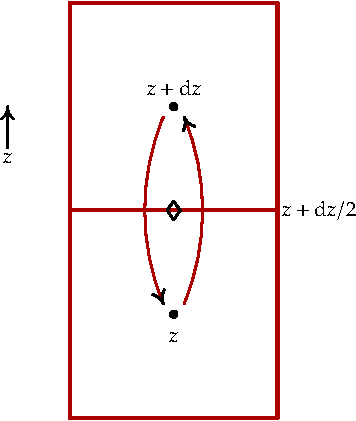
\includegraphics{./mfpic_figs/cvmix_stability.pdf}}
\caption[Parcel displacements for gravitational stability calculation]
{Illustration of how parcels are displaced when checking for the
  gravitational stability. As for the discrete column shown in Figure
  \ref{fig:cvmix_discrete_vertical}, we assume knowledge of the tracer
  and pressure values at the tracer points $z$ and
  $z+\mathrm{d}z$. Two displacements are considered: one vertically up
  and one vertically down.  The notation corresponds on the discrete
  grid of Figure \ref{fig:cvmix_discrete_vertical}, where
  $z+\mathrm{d}z$ in the present figure corresponds to an interface
  depth {\tt zw(kw)}; the deeper point at $z$ corresponds to the
  tracer point {\tt zt(kt+1)}; and the shallower point $z+\mathrm{d}z$
  corresponds to the tracer point {\tt zt(kt)}.}
\label{fig:cvmix_stability}
\end{center}
\end{figure}


\subsubsection{Stability to downward displacements from a shallower reference point}

We now determine the gravitational stability of fluid to displacements
from a shallow reference point $z^{*} = z + \mathrm{d}z$ downward to
$z$, which requires the calculation
\begin{equation}
\begin{split}
\rho(z)  - \rho(z)_{\mbox{\tiny adiabatic/isohaline}}  
&= 
 \rho[ \Theta(z), S(z), p(z)]
-
\rho[ \Theta(z+\mathrm{d}z), S(z+\mathrm{d}z), p(z)]
\\
 &=
 \rho[ \Theta(z^{*}-\mathrm{d}z), S(z^{*}-\mathrm{d}z), p(z)]
-
\rho[ \Theta(z^{*}), S(z^{*}), p(z)]
\\
&\approx 
 -\rho \, \mathrm{d}z \, \left[ 
   -\alpha \, \left( \frac{\partial \Theta}{\partial z} \right )
  + \beta \, \left( \frac{\partial S}{\partial z} \right) \right]
 \\
&=
\left( \frac{\rho \, \mathrm{d}z}{g} \right) \, N^{2},
\end{split}
\label{eq:inifinitesimal-delta-rho-elements-downward}
\end{equation}
where terms in the final two equalities are evaluated at the shallow
reference point $z^{*} = z + \mathrm{d}z$.  Following equation
(\ref{eq:inifinitesimal-delta-rho-elements-upwards2}), we introduce the
full squared buoyancy frequency
\begin{equation}
\begin{split}
 N^{2}_{\mbox{\scriptsize full}}(z +\mathrm{d}z \rightarrow z) &\equiv 
 \left( \frac{g \, [ \rho(z)  - \rho(z)_{\mbox{\tiny adiabatic/isohaline}} ] } {\rho(z+\mathrm{d}z) \, \mathrm{d}z} \right).
\end{split}
\label{eq:inifinitesimal-delta-rho-elements-downwards}
\end{equation}



\subsubsection{Combined displacements to approximate gravitational stability at
  interface depth}

Let us summarize the two previous results.  Again, we have two tracer
points at depths $z$ and $z+\mathrm{d}z$.  Gravitational stability can
be probed in two separate ways. First we consider the deeper depth $z$
as a reference point and displace parcels vertically upward to
$z+\mathrm{d}z$.  This calculation leads to the squared buoyancy
frequency at the reference point $z$
\begin{equation}
\begin{split}
 N^{2}_{\mbox{\scriptsize full}}(z \rightarrow z + \mathrm{d}z)
 &=
 -\left(  \frac{g \, [\rho(z+\mathrm{d} z)  - \rho(z+\mathrm{d} z)_{\mbox{\tiny adiabatic/isohaline}} ]}{\rho(z)   \, \mathrm{d}z } \right)
\\
&=
 -\frac{g}{\rho(z)}  \left( 
 \frac{\rho[ \Theta(z + \mathrm{d} z), S(z + \mathrm{d} z), p(z + \mathrm{d} z)]
-
\rho[ \Theta(z), S(z), p(z + \mathrm{d}z)]
}{\mathrm{d}z}
\right).
\end{split}
\label{eq:inifinitesimal-delta-rho-elements-upwards-summary}
\end{equation}
We next the shallower depth $z+\mathrm{d}z$ as a reference point and
displace parcels vertically downward to $z$.  This calculation leads
to the squared buoyancy frequency at the reference point
$z+\mathrm{d}z$
\begin{equation}
\begin{split}
 N^{2}_{\mbox{\scriptsize full}}(z + \mathrm{d}z \rightarrow z)
 &=
 \left(  \frac{g \, [\rho(z)  - \rho(z)_{\mbox{\tiny adiabatic/isohaline}}  ]}{\rho(z+\mathrm{d}z)   \, \mathrm{d}z } \right)  
 \\
 &=
 \frac{g}{\rho(z+\mathrm{d}z)}  \left( 
 \frac{ \rho[ \Theta(z), S(z), p(z)]-
 \rho[ \Theta(z+\mathrm{d}z), S(z+\mathrm{d}z), p(z)]
  }{\mathrm{d}z}
\right).
\end{split}
\label{eq:inifinitesimal-delta-rho-elements-downward-summary}
\end{equation}
We now use these two results to render an approximation to the squared
buoyancy frequency at the interface point $z + \mathrm{d}z/2$, which
is where the discrete calculation requires the stability to be
estimated (Section \ref{subsubsection:numerics-buoyancy-frequency}).
For this purpose, we take the average to yield an expression in terms
of density differences \small
\begin{equation}
\begin{split}
N^{2}_{\mbox{\scriptsize full}}(z+\mathrm{d}z/2) 
 &\equiv 
 \frac{N^{2}_{\mbox{\scriptsize full}}(z \rightarrow z + \mathrm{d}z) + N^{2}_{\mbox{\scriptsize full}}(z + \mathrm{d}z \rightarrow z)}{2}
\\
&= \frac{g}{2} 
  \left( 
 -\frac{
    \rho[ \Theta(z + \mathrm{d} z), S(z + \mathrm{d} z), p(z + \mathrm{d} z)]
  -\rho[ \Theta(z), S(z), p(z + \mathrm{d}z)]
  }{\rho(z) \, \mathrm{d}z}
 \; + \; 
 \frac{ \rho[ \Theta(z), S(z), p(z)]-
 \rho[ \Theta(z+\mathrm{d}z), S(z+\mathrm{d}z), p(z)]
  }{\rho(z+\mathrm{d}z) \, \mathrm{d}z}
 \right).
\end{split}
\label{eq:n2-in-terms-of-density-differences}
\end{equation}
\normalsize As a sanity check, note that if the density is independent
of pressure, and we replace densities in the denominator with the
constant reference density $\rho_{o}$, we have the familiar simplified
result
\begin{equation}
N^{2}(z+\mathrm{d}z/2) = -\frac{g}{\rho_{o}} 
  \left( 
 \frac{
    \rho[ \Theta(z + \mathrm{d} z), S(z + \mathrm{d} z)]
  -\rho[ \Theta(z), S(z)]
  }{\mathrm{d}z}
 \right)    \qquad   \mbox{density independent of pressure}.
\end{equation}


\subsubsection{Linear approximation: not recommended in general}

Instead of computing the full buoyancy frequency in terms of density
differences, one may choose to make a linearization of the expansion
following equation (\ref{eq:buoyancy-frequency-elements}), in which we
write
\begin{equation}
\begin{split}
N^{2}_{\mbox{\scriptsize linear}} (z+\mathrm{d}z/2) 
&\equiv \frac{N^{2}_{\mbox{\scriptsize linear}} (z) + N^{2}_{\mbox{\scriptsize linear}} (z+\mathrm{d}z)}{2}
\\
&= 
 g \, \left( \overline{\alpha}^{z}  \, \frac{\partial \Theta}{\partial z} 
               -\overline{\beta}^{z} \,  \frac{\partial S}{\partial z} \right),
\end{split}
\label{eq:n2-in-terms-of-tracers}
\end{equation} 
where we introduced the vertical averaging operator to bring the
expansion coefficients from the tracer point to the interface
\begin{equation}
  \overline{\alpha}(z+\mathrm{d}z/2) = \frac{\alpha(z) + \alpha(z+\mathrm{d}z)}{2}.
\end{equation}
The vertical tracer derivatives are naturally placed on the vertical
cell interface.  Contrary to the density difference approach of
equation (\ref{eq:n2-in-terms-of-density-differences}), the expression
(\ref{eq:n2-in-terms-of-tracers}) requires no non-standard
calculations of the equation of state.  What it does require is
calculation of the thermal expansion coefficients, with that
calculation also used for neutral physics.  So the expression
(\ref{eq:n2-in-terms-of-tracers}) may be somewhat more efficient.
Nonetheless, when used as a measure of gravitational stability, the
expression (\ref{eq:n2-in-terms-of-density-differences}) makes less
assumptions about our ability to truncate the Taylor series at the
leading order.  This truncation may become problematic particularly in
high latitudes where the equation of state can become quite nonlinear.
Hence, we generally do not recommend use of the expression
(\ref{eq:n2-in-terms-of-tracers}).


\subsubsection{Discrete calculation of the squared buoyancy frequency}
\label{subsubsection:numerics-buoyancy-frequency}

CVMix modules do {\it not} compute the buoyancy frequency.  Rather,
the calling model does and then passes $N^{2}$ to CVMix. Nonetheless,
CVMix modules must assume a placement for the buoyancy frequency, with
the following choice made:
\begin{quote}
  {\sf CVMix modules assume the squared buoyancy frequency, $N^{2}$,
      lives at the vertical interface of tracer cells, following the
      convention given by Figure \ref{fig:cvmix_discrete_vertical}.}
\end{quote}
We now write the buoyancy frequency expression
(\ref{eq:n2-in-terms-of-density-differences}) in terms of discrete
indices for ready incorporation into a numerical model, in which we have 
\small
\begin{equation}
N^{2}({\tt kw}) = 
 \frac{g}{2} 
  \left( 
 -\frac{
    \rho[ \Theta( {\tt kt}), S( {\tt kt}), p( {\tt kt})]
  -\rho[ \Theta( {\tt kt+1} ), S({\tt kt +1} ), p( {\tt kt} )]
  }{\rho({\tt kt+1} ) \,  {\tt dzw(kw)} }
 \; +  \; 
 \frac{ \rho[ \Theta({\tt kt+1}), S({\tt kt+1}), p({\tt kt+1})]-
 \rho[ \Theta({\tt kt} ), S( {\tt kt}), p({\tt kt+1})]
  }{\rho( {\tt kt}) \, {\tt dzw(kw)}  }
 \right).
\label{eq:n2-in-terms-of-density-differences-discrete}
\end{equation}
\normalsize Note that by referring to Figures
\ref{fig:cvmix_discrete_vertical} and \ref{fig:cvmix_stability}, we
see that the discrete label {\tt kt} corresponds to the shallower
point $z+\mathrm{d}z$, whereas {\tt kt+1} corresponds to the deeper
point $z$.  This correspondence is made when converting equation
(\ref{eq:n2-in-terms-of-density-differences}) to
equation (\ref{eq:n2-in-terms-of-density-differences-discrete}).


\section{Gradient Richardson number}
\label{section:gradient-richardson-number-elements}

The gradient Richardson number measures the ratio of the stabilizing
effects from buoyancy stratification to the destabilizing effects from
vertical shear
\begin{equation}
  \mbox{Ri}= \frac{N^{2} }{ |\partial_{z} \, {\bf u}|^{2} }.
\label{eq:flux-Richardson-elements}
\end{equation}
In this equation, $N^{2}$ is the squared buoyancy frequency, whose
discrete calculation was detailed in Section
\ref{subsubsection:numerics-buoyancy-frequency}.  The denominator
contains the squared vertical shear of the horizontal velocity,
$|\partial_{z} \, {\bf u}|^{2}$.  When the Richardson number is small,
say below 1/4 as in \cite{miles1961}, the flow tends toward a
turbulent state via production of Kelvin-Helmholz
instabilities.\footnote{The critical Richardson number, below which
  instabilities are enabled, may need to be artificially set larger
  than the canonical 1/4 when considering discrete approximations to
  the velocity shear.  The reason is that we are unable to precisely
  compute the vertical shear on a finite grid.}  Consequently, many
vertical mixing schemes make use of the Richardson number, such as the
shear mixing schemes presented in Chapter \ref{chapter:cvmix_shear}.
Additionally, the KPP boundary layer scheme (Chapter
\ref{chapter:cvmix_kpp}) makes use of a bulk Richardson number used to
define properties of the surface planetary boundary layer (Section
\ref{subsection:kpp-obl-thickness}).

As for the squared buoyancy frequency $N^{2}$, the CVMix modules do
{\it not} compute a Richardson number, since details of this
calculation depend on choices regarding the grid layout in the ocean
model.  Rather, the Richardson number is an input to CVMix modules.
CVMix modules assume a placement for the Richardson number, with the
following choice made:
\begin{quote}
  {\sf The gradient Richardson number, $\mbox{Ri}$, is an input to
    CVMix modules.  CVMix modules assume the gradient Richardson
    number lives at the vertical interface of tracer cells, following
    the convention given by Figure
    \ref{fig:cvmix_discrete_vertical}.}
\end{quote}

Staggering of tracer and velocity fields on a discrete grid leads to
ambiguity for how to compute a discrete Richardson number.  The issue
is the squared buoyancy frequency in the numerator naturally lives at
the vertical interface between tracer grids (Section
\ref{subsubsection:numerics-buoyancy-frequency}), whereas the
horizontal positioning for the denominator depends on the chosen
horizontal staggering of velocity.  We detail here some possible
methods for the B-grid and C-grid.  Unstructured grids used by
MPAS-ocean require further considerations.  Each grid involves
averaging operations specific to the grid in order to compute the
shear.  There are even further methods available if we choose a
different discrete placement of $N^{2}$ beyond that discussed in
Section \ref{subsubsection:numerics-buoyancy-frequency}.


\subsection{Considerations for the B-grid}
\label{subsection:b-grid-richardson-number}

Figure \ref{fig:b-grid} illustrates the horizontal arrangement of
prognostic model fields used with the B-grid. The B-grid places both
horizontal prognostic velocity components at the same point, the
corner of the tracer cell.  This placement is natural when computing
the Coriolis Force.  However, it is unnatural for computation of
advective tracer transport or the horizontal pressure gradient force
acting on velocity.  The need to perform an averaging operation when
computing the horizontal pressure gradient leads to the computational
mode associated with gravity waves on the B-grid (\cite{Mesinger1973},
\cite{KillworthFreesurf1991}, \cite{MOM3manual},
\cite{GriffiesPacSchmidtBalaji2001}, and Section 12.9 of
\cite{SMGbook}).

\begin{figure}
\begin{center}
\resizebox{7cm}{!}{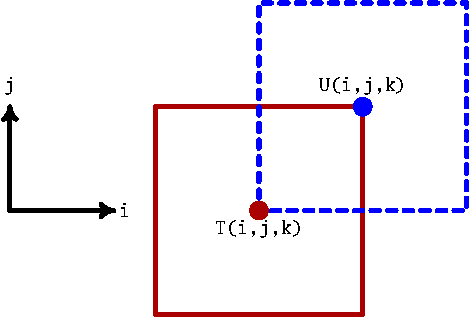
\includegraphics{./mfpic_figs/B_grid.pdf}}
\caption[Placement of fields onto the B-grid] {Illustration of how
  fields are placed on the horizontal B-grid using a {\it northeast
    convention}.  Velocity points {\tt U(i,j,k)} are placed to the
  northeast of tracer points {\tt T(i,j,k)}.  Both horizontal velocity
  components $u_{i,j,k}$ and $v_{i,j,k}$ are placed at the velocity
  point {\tt U(i,j,k)}.  Both the tracer point and velocity point have
  a corresponding grid cell region, denoted by the solid and dashed
  squares.}
\label{fig:b-grid}
\end{center}
\end{figure}

We present here some methods for computing the squared vertical shear
of the horizontal velocity on the B-grid, and thus methods for
computing the Richardson number.
\begin{itemize}

\item {\sc T-grid average of U-grid velocity}: The first approach
  computes a horizontal average of the velocity field to place it onto
  the T-grid, and then computes the vertical derivative and its
  square.  The 4-point horizontal average to compute a T-grid velocity
  is written
\begin{equation}
  {\bf u}^{\mbox{\tiny T}}  = \overline{\bf u}^{x,y}.
\end{equation}
Note that this, and all, four point averages do {\it not} include land
points. We next compute the squared vertical shear with the T-grid
horizontal velocity for use in the Richardson number calculation
\begin{equation}
    \mbox{Ri}^{(\mbox{\tiny Ba})} = \frac{N^{2}} { \left| \frac{\partial {\bf u}^{\mbox{\tiny T}}}{\partial z} \right|^{2} }.
\end{equation}

\item {\sc T-grid average of U-grid shear}: A slight modification of
  the $\mbox{Ri}^{(\mbox{\tiny Ba})}$ calculation takes the T-grid
  horizontal average of the U-grid shear
\begin{equation}
  \left( \frac{\partial {\bf u}}{\partial z} \right)^{\mbox{\tiny T}}
  = \overline{ \left( \frac{\partial {\bf u}}{\partial z} \right)}^{x,y},
\end{equation}
and then computes the square so that
\begin{equation}
    \mbox{Ri}^{(\mbox{\tiny Bb})} = \frac{N^{2}} { \left|  \left( \frac{\partial {\bf u}}{\partial z} \right)^{\mbox{\tiny T}} \right|^{2} }.
\end{equation}
With uniform vertical grid spacing, the two Richardson number
calculations are the same
\begin{equation}
 \mbox{Ri}^{(\mbox{\tiny Ba})} = \mbox{Ri}^{(\mbox{\tiny Bb})}  \qquad \mbox{uniform vertical grid spacing.}
\end{equation}

\item {\sc T-grid average of squared U-grid shear}: The third method
  computes the squared shear on the original U-grid, and then averages
  the squared shears onto the T-grid
\begin{equation}
  \left( \left| \frac{\partial {\bf u}}{\partial z} \right|^{2} \right)^{\mbox{\tiny T}}
  = \overline{  \left( \left| \frac{\partial u}{\partial z}  \right|^{2}  
     +  \left| \frac{\partial v}{\partial z}  \right|^{2}  \right)  }^{x,y},
\end{equation}
so that 
\begin{equation}
    \mbox{Ri}^{(\mbox{\tiny Bc})} = \frac{N^{2}} { \left( \left| \frac{\partial {\bf u}}{\partial z} \right|^{2} \right)^{\mbox{\tiny T}}}.
\end{equation}

\end{itemize}



\subsection{Considerations for the C-grid}
\label{subsection:c-grid-richardson-number}

Figure \ref{fig:c-grid} illustrates the horizontal arrangement of
prognostic model fields used with the C-grid. The C-grid places the
zonal velocity component on the zonal tracer cell face, and meridional
velocity component on the meridional tracer cell face.  This placement
is suited for computation of advective tracer transport.  It is also
suited for computing the stress tensor and the horizontal pressure
gradient force acting on velocity components.  However, it is not
natural for computation of the Coriolis Force.  The need to perform an
averaging operation to compute the Coriolis Force leads to the
presence of a computational null mode associated with geostrophically
balanced flow \citep{Adcroftetal1999}.

\begin{figure}
\begin{center}
\resizebox{7cm}{!}{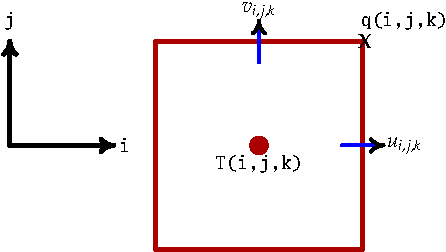
\includegraphics{./mfpic_figs/C_grid.pdf}}
\caption[Placement of fields onto the C-grid] {Illustration of how
  fields are placed on the horizontal C-grid.  We illustrate here the
  convention that the zonal velocity component $u_{i,j,k}$ sits at the
  east face of the tracer cell {\tt T(i,j)}, and the meridional
  velocity component $v_{i,j,k}$ sits at the north face of the tracer
  cell {\tt T(i,j,k)}.  This convention follows the {\it northeast}
  convention also used for the B-grid.}
\label{fig:c-grid}
\end{center}
\end{figure}


We present here some methods for computing the squared vertical shear
of the horizontal velocity on the C-grid, and thus methods for
computing the Richardson number. 
\begin{itemize}

\item {\sc T-grid average of u,v-grid velocity components}: The first
  approach considered computes a horizontal average of the $u,v$
  velocity components to place both onto the T-grid, and then computes
  the vertical derivative and its square.  The horizontal averaging
  requires a two-point average so that 
\begin{equation}
  (u^{\mbox{\tiny T}}, v^{\mbox{\tiny T}}) = (\overline{u}^{x}, \overline{v}^{y}).
\end{equation}
As for the B-grid averaging considered in Section
\ref{subsection:b-grid-richardson-number}, all averages considered
here do {\it not} include land points. The squared vertical shear with
the T-grid horizontal velocity is then used for the Richardson number
calculation
\begin{align}
 \left| \frac{\partial {\bf u}^{\mbox{\tiny T}}}{\partial z} \right|^{2}
 &= \left( \frac{\partial \overline{u}^{x}}{\partial z} \right)^{2} 
     +
     \left( \frac{\partial \overline{v}^{y}}{\partial z} \right)^{2} 
\\
    \mbox{Ri}^{(\mbox{\tiny Ca})} &= \frac{N^{2}} { \left| \frac{\partial {\bf u}^{\mbox{\tiny T}}}{\partial z} \right|^{2} }.
\end{align}


\item {\sc T-grid average of u,v-grid shear}: A slight modification of
  the $\mbox{Ri}^{(\mbox{\tiny Ca})}$ calculation takes the T-grid
  horizontal average of the u,v-grid shear
\begin{equation}
  \left( \frac{\partial {\bf u}}{\partial z} \right)^{\mbox{\tiny T}}
  = 
  \left[  \overline{ \left( \frac{\partial u}{\partial z} \right)}^{x}, \overline{ \left( \frac{\partial v}{\partial z} \right)}^{y}
   \right],
\end{equation}
and then computes the square so that
\begin{equation}
    \mbox{Ri}^{(\mbox{\tiny Cb})} = \frac{N^{2}} { \left|  \left( \frac{\partial {\bf u}}{\partial z} \right)^{\mbox{\tiny T}} \right|^{2} }.
\end{equation}
With uniform vertical grid spacing, the two Richardson number
calculations are the same
\begin{equation}
 \mbox{Ri}^{(\mbox{\tiny Ca})} = \mbox{Ri}^{(\mbox{\tiny Cb})}  \qquad \mbox{uniform vertical grid spacing.}
\end{equation}

\item {\sc T-grid average of squared u,v-grid shear}: The third method
  computes the squared shear on the original u,v-grid, and then averages
  the squared shears onto the T-grid
\begin{equation}
  \left( \left| \frac{\partial {\bf u}}{\partial z} \right|^{2} \right)^{\mbox{\tiny T}}
  = \overline{  \left| \frac{\partial u}{\partial z} \right|^{2}   }^{x}
    +
   \; \; \overline{ \left| \frac{\partial v}{\partial z} \right|^{2}  }^{y}
\end{equation}
so that 
\begin{equation}
    \mbox{Ri}^{(\mbox{\tiny Bc})} = \frac{N^{2}} { \left( \left| \frac{\partial {\bf u}}{\partial z} \right|^{2} \right)^{\mbox{\tiny T}}}.
\end{equation}


\end{itemize}


\subsection{Considerations for unstructured grids used by MPAS-ocean}
\label{subsection:mpas-grid-richardson-number}

To be completed.  

